\documentclass[../root]{subfiles}
\graphicspath{{_images/}{../_images/}}


\begin{document}

    \chapter{Testing for altruism and social pressure in charitable giving}

    \begin{shortsummary}
        \begin{itemize}
            \item \authoryear{Dellavigna2012}
            \item \RQ{Door-to-Doorの募金活動は寄付者の厚生を下げるのかどうか?}
            \item \answer{シカゴ近辺の町で行った大規模なフィールド実験の結果とそれを用いた構造推定}
            \item \result{個人の寄付動機は利他性ではなくsocial pressureがあるため、募金活動は寄付者の厚生を下げる}
        \end{itemize}
    \end{shortsummary}

    \section{Research Question}

    \begin{itemize}
        \item 寄付のモチベーションを大きく二つに大別して考える
        \begin{itemize}
            \item Altruism:寄付することに効用を得る、Supply-driven、寄付は効用を最大にする
            \item Social pressure:勧誘員が寄付するように心理的な圧力をかける、Demand-driven、寄付は寄付者の効用を下げる
        \end{itemize}
        \item この研究は、寄付行為が寄付者の厚生を上げるか下げるのかをフィールド実験(シカゴ近辺の7,668世帯)で確かめる
        \begin{itemize}
            \item 3つのトリートメント
            \begin{enumerate}
                \item ドアノブに翌日の同じ時間に寄付を求める広告をかける
                \item その広告の中に「Do not disturb」のチェックボックスを加える⇒チェックを加えたら、勧誘員は来ない
                \item 広告をかけずに、直接寄付を求める
            \end{enumerate}
            \item 利他効用が動機ならば、広告は勧誘員が来る時間帯に家にいる可能性と寄付額を増やす(\textbf{sorting into staying at home})
            \item social pressureが動機ならば、広告は勧誘員が来る時間帯に家にいる可能性と寄付額を減らす(\textbf{sorting out of opening the door})
            \item 主な結果:Social pressureの役割が強かったが、altruismの役割がないわけでない
            \begin{enumerate}
                \item 広告の提供は勧誘員が来た時にドアを開ける頻度を減らした(とくにチェックボックスを加えたとき)
                \item チェックボックスをつけた広告は寄付額を減らした。これは10\$未満の寄付者を増やしたことに起因する
                \item メールやインターネットなどの代替手段を用いた寄付に対する効果はない
            \end{enumerate}
        \end{itemize}
        \item この実験に追加したsurveyを行い、structural estimationでwelfare effectを推定
        \begin{itemize}
            \item 重要なパラメータ:利他効用を持つ人の割合、利他効用関数のcurvature、勧誘員に寄付しないと回答するときのsocial pressure cost
            \item 結果:door-to-door campaignは寄付者のwelfareを下げた
            \begin{enumerate}
                \item potential giversの75\%が利他性的でないが、利他選好に大きな異質性がある
                \item social pressure costは\$3.75(in-state charity)と\$1.44(out-of-state charity)
                \item welfareは\$1.10(in-state charity)と\$0.44(out-of-state charity)だけ下げた
            \end{enumerate}
            \item 寄付者のwelfareを下げているが、レシピエントのwelfareを高めている可能性があるので、overall welfare effectは増加しているかもしれない
        \end{itemize}
    \end{itemize}

    \section{Model}

    \subsection{Settings}

    \begin{itemize}
        \item 確率$r$である世帯がフライヤーに気づく(外生)
        \item 意思決定は以下のシーケンスに沿って行われる
        \begin{enumerate}
            \item 寄付者は勧誘員が来たとき、確率$h$でそれに応対する
            \begin{itemize}
                \item もともとの応対確率は$h0$であり、フライヤーに気づくことでその確率を変えられる(ただし、コストがかかる)
            \end{itemize}
            \item 応対したかどうかによって、寄付者は最適な寄付額$(g, g_m)$を決める
            \begin{itemize}
                \item $g$は勧誘員に直接寄付する額、$g_m$はインターネットなどの別手段で勧誘員が所属する慈善団体に寄付する額
                \item $g_m$はoverhead costがかかり、最終的に慈善団体が受け取る額は$\theta*g_m$
                \item $g_m$には追加コストがあるので、勧誘員に応対するならば、$g_m = 0$となる。したがって、$g_m$は勧誘員に直接寄付できなかった人のための代替手段。
            \end{itemize}
        \end{enumerate}
    \end{itemize}
    
    \begin{itemize}
        \item 効用関数の定義
        \begin{align*}
            U(g, g_m) = u(W - g - g_m) + av(g + \theta g_m, G_{-i}) - S(g)
        \end{align*}
        \begin{itemize}
            \item $u$:concave utility function of private consumption ($W$ is pre-giving wealth)
            \item $v$:giving utility function (impure altruismやspitefulを考慮できる、$a$は利他性の強度)
            \item $s$:social pressure cost function, $s(g) = S(gs - g) 1(g < gs)$. $g_s$以上寄付するとsocial pressureを受けないので、これはある種の社会的な規範ともとれる 
        \end{itemize}
        \item 第二ステージにおける各最適な行動を所与として、応対確率hを以下のように決める
        \begin{align*}
            \max_{h \in [0,1]} h[u(W-g^*) + a v(g^*, G_{-i}) - s(g^*)] + (1-h)[u(W - g^*_m) + av(\theta g^*_m, G_{-i})] - c(h)
        \end{align*}
    \end{itemize}

    \subsection{Solutions}

    \begin{figure}[t]
        \centering
        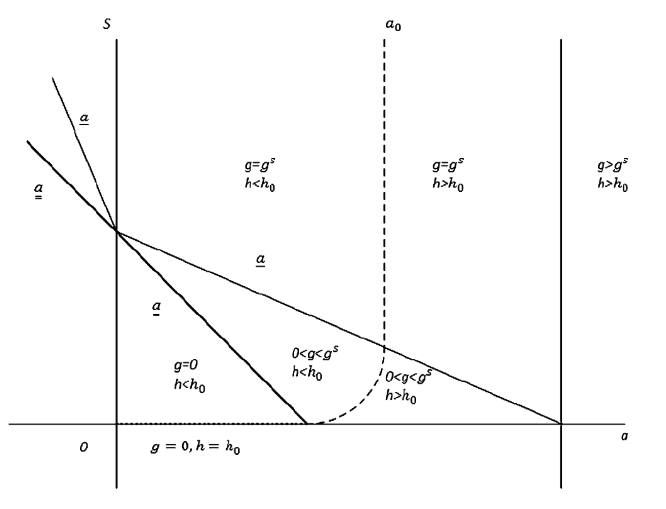
\includegraphics[width = .8\linewidth]{0821kato/fig1_2.png}
        \caption{Regions of Giving and Probability of Home Presence}
        \label{}
    \end{figure}

    \begin{itemize}
        \item 寄付額は利他性の程度の増加関数である。
        \begin{itemize}
            \item とくに、利他性の強度が十分に高いと、social pressureに関わらず社会規範を超えた寄付をする
            \item 社会規範を超えた寄付は完全に利他性によるものだが、社会規範を下回る寄付は利他性とsocial pressureによるもの
        \end{itemize}
        \item 応対確率は利他性の程度の弱増加関数である
        \begin{itemize}
            \item 利他性の強度が強いほど、フライヤーによって応対確率を高めるように調整する(seeking)
            \item social pressureがないとき、利他性が低い人がフライヤーによって応対確率を低めるように調整するという行動(avoiding)は観察されない
        \end{itemize}
    \end{itemize}

    \subsection{Opt-out Policy}

    \begin{itemize}
        \item "Do not disturb"のチェックボックスによって、個人は応対確率を0に下げることをコストレスに行うことができる。
        \begin{itemize}
            \item $c(0) = 0$, $c(h) > 0$ for $h > 0$
            \item 重要:社会的イメージやセルフイメージをmotivationとしているならば、この政策を利用して、h = 0を取ることはむしろコストとなる(勧誘員がこれに気づいて利他性のタイプを推測できるから)
        \end{itemize}
        \item social pressureがないとき、この政策の導入は応対確率の最適行動に影響を与えない
        \item social pressureがあるとき、利他性の強度が低い人はこの政策を利用するが、利他性が高い人はこの政策を利用せずに、行動も変えない
    \end{itemize}

    \subsection{Testable Predictions}

    \begin{itemize}
        \item 二つのケースで予測を導出している
        \begin{enumerate}
            \item Altruism and No social pressure:S = 0であり、利他性の強度はある程度高い
            \item Social pressure and Limited Altruism:S > 0であり、利他性の強度がある程度高い人はいない
        \end{enumerate}
        \item 以下の6つの検証可能な予測を出している
        \begin{enumerate}
            \item 応対確率(家にいる確率):Altruism and No social pressureのとき、(flyer)=(opt-out flyer)> (no flyer)である。Social pressure and Limited altruismのとき、(no flyer) > (flyer) > (opt-out flyer)
            \item unconditional giving prob:Altruism and No social pressureのとき、(flyer) = (opt-out flyer) > (no flyer)である。Social pressure and Limited altruismのとき、(no flyer) > (flyer) > (opt-out flyer)
            \item giving prob conditional on being at home:$\min\{ \text{(flyer), (opt-out flyer)} \} > \text{(no flyer)}$
            \item unconditional large giving prob ($g > g_s$):(flyer) = (opt-out flyer) > (no flyer)
            \item unconditional small giving prob ($g_s > g$):(flyer) = (opt-out flyer) if S = 0; otherwise (flyer) > (opt-out flyer)
            \item unconditional via-mail giving prob:(opt-out flyer) > (flyer) > (no flyer) = 0
        \end{enumerate}
    \end{itemize}

    \section{Experimental Design}

    \begin{figure}[t]
        \centering
        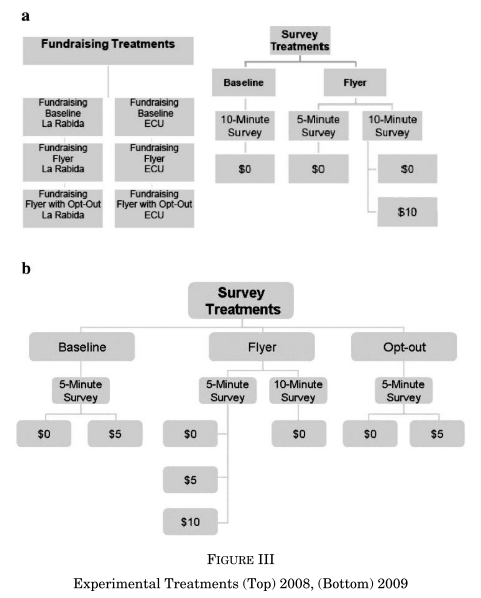
\includegraphics[width = .5\linewidth]{0821kato/fig3_2.png}
        %\caption{}
        \label{}
    \end{figure}

    \begin{figure}[t]
        \centering
        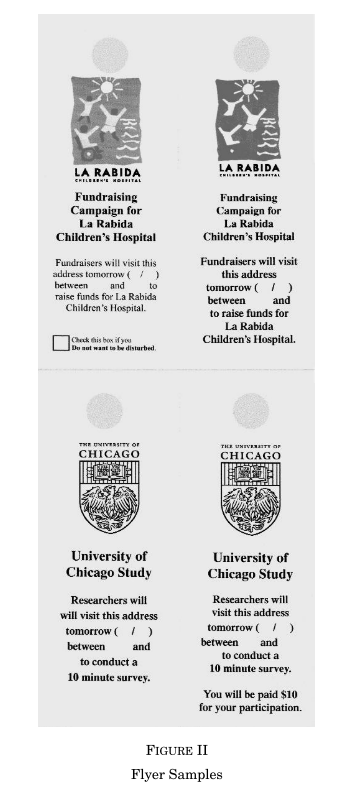
\includegraphics[width = .5\linewidth]{0821kato/fig2_2.png}
        %\caption{}
        \label{}
    \end{figure}
    
    \begin{itemize}
        \item La Rabida Children's Hospital (in-state charity contributes to child health) と East Carolina Hazard Center (out-state charity) の協力
        \item Solicitor:92名を大学で雇った(ほとんどはシカゴ大学の学部生、時給\$9.50)
        \begin{itemize}
            \item トレーニングを受けて、実際の調査に参加する
            \item 1時間で25世帯を回るように設計、従事時間は4時間もしくは6時間
            \item トリートメントの詳細を知らない(その家にflyerがあるかどうかも知らない)
            \item 応対してくれたら、決められたスクリプトを読み上げて寄付を求める
        \end{itemize}
        \item locations: wealthy towns around Chicago
        \begin{itemize}
            \item この地域において、door-to-door campaignはよくある話であり、La Rabidaの方が人気
        \end{itemize}
        \item Charity treatment: 2008年の土日
        \begin{itemize}
            \item 4/27 ~ 6/1:$\text{two charities}\times\text{three treatments}$
            \item 7/13 ~ 8/23:$\text{La Rabida} \times \{\text{no flyer, flyer}\}$
            \item 9/6 ~ 10/18:$\text{two charities (over-weighted ECU)} \times \text{all treatments}$
        \end{itemize}
        \item Survey treatment: 2008年4月の土日、2008年10月の土日、2009年4月の土日、2009年11月の土日(詳しい日付なし)
        \begin{itemize}
            \item $\text{flyer treatments}\times\text{incentive}\times\text{duration}$
            \item incentiveは調査に対する謝礼(\$0, \$5, \$10)で、durationは調査にかかる時間(5min, 10min)
            \item flyer もしくは opt-out flyer treatmentの場合、incentiveとdurationの情報を与えられる。no flyer treatmentの場合、調査員が参加するか尋ねる前に伝える。
            \item 意識調査を通じて、在宅の弾力性とインセンティブに対する反応率を調べる⇒この値を使い構造推定を行う
            \item 意識調査の中身にはそこまで興味ない
        \end{itemize}
        \item between-subjects treatment: 各調査期において、勧誘員の時間帯×street levelでランダム化
    \end{itemize}

    

    \clearpage
    \section{Reduced-form Results}

    \subsection{記述統計}

    \begin{figure}[h]
        \centering
        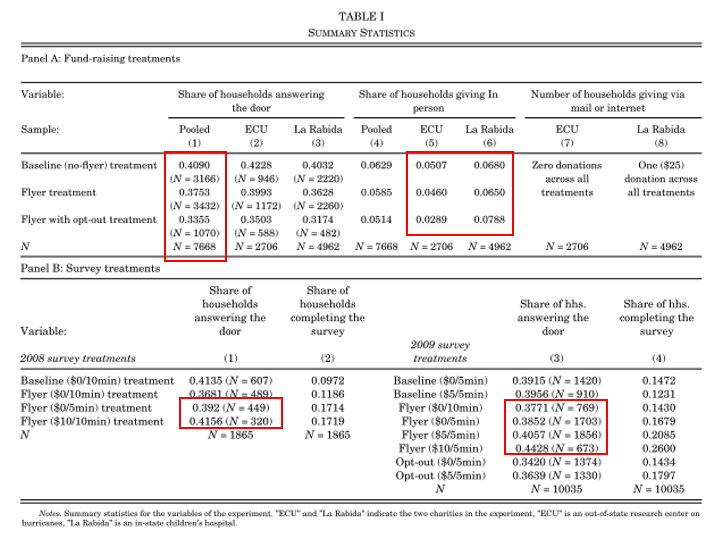
\includegraphics[width = .8\linewidth]{0821kato/fig4_2.png}
        %\caption{}
        \label{}
    \end{figure}

    \begin{itemize}
        \item Charity treatment
        \begin{itemize}
            \item 応答確率は(no flyer) > (flyer) > (opt-out flyer)
            \item 寄付確率は(La Rabida) > (ECU)
            \item ECU charityについて、寄付確率は(no flyer) > (flyer) > (opt-out flyer)
            \item La Rabida charityについて、寄付確率は(no flyer) = (flyer) < (opt-out flyer)
        \end{itemize}
        \item Survey treatment
        \begin{itemize}
            \item どちらの年の調査も、時間が短いほど、またインセンティブが高いほど、応答確率が高くなる
        \end{itemize}
        \item 時期によってトリートメントを行っていないことがあるので、以下の分析は固定効果を加えたうえでの推定値を使って、各アウトカムのfrequencyを計算している。
    \end{itemize}

    \subsection{応答確率}

    \begin{figure}[h]
        \centering
        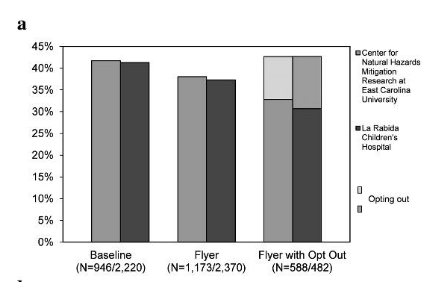
\includegraphics[width = .5\linewidth]{0821kato/fig5_2.png}
        \caption{Frequency of Answering the Door}
        \label{}
    \end{figure}

    \begin{itemize}
        \item no flyer から flyer になると応答確率はおよそ4\%下がり、flyerからopt-out flyerになるとその確率はさらに5-6\%下がる
        \begin{itemize}
            \item social pressureのエビデンス:訪問することを知ったら、そこから逃れるように行動する
            \item opt-out flyerのチェックボックスにチェックを入れた人の割合はおよそ10%
        \end{itemize}
    \end{itemize}

    \subsection{条件なしの寄付確率}

    \begin{figure}[h]
        \centering
        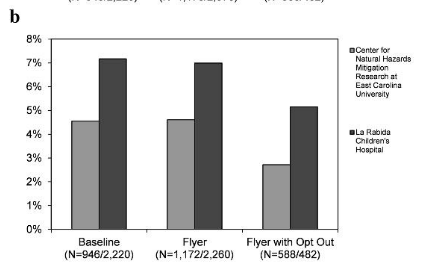
\includegraphics[width = .5\linewidth]{0821kato/fig6_2.png}
        \caption{Frequency of Unconditional Giving}
        \label{}
    \end{figure}

    \begin{itemize}
        \item no flyerとflyerの寄付確率はほとんど同じだが、opt-out flyerの寄付確率はおよそ2\%下がる
        \begin{itemize}
            \item no flyer = flyer:利他性とsocial pressureが与える影響がほとんど同じならば、この結果は説明がつく
            \item flyer > opt-out flyer:social pressureの影響といえる。このトリートメントの差は回避行動コストの差だけなので、利他性が主要因であれば、この二つのトリートメント間に差はないはず
        \end{itemize}
    \end{itemize}

    \subsection{応答した人で条件づけた寄付確率}

    \begin{figure}[h]
        \centering
        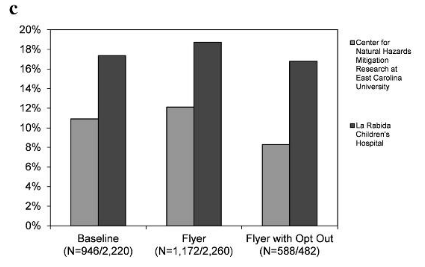
\includegraphics[width = .5\linewidth]{0821kato/fig7_2.png}
        \caption{Frequency of Giving Conditional on Answering the Door}
        \label{}
    \end{figure}

    \begin{itemize}
        \item flyer condは条件付き寄付確率を高めたが、opt-out flyer condはそれを低めた(非有意)
        \begin{itemize}
            \item 前者の結果は理論予測と整合的だが、後者はそうでない
        \end{itemize}
    \end{itemize}

    \subsection{条件なし寄付金額}

    \begin{figure}[h]
        \centering
        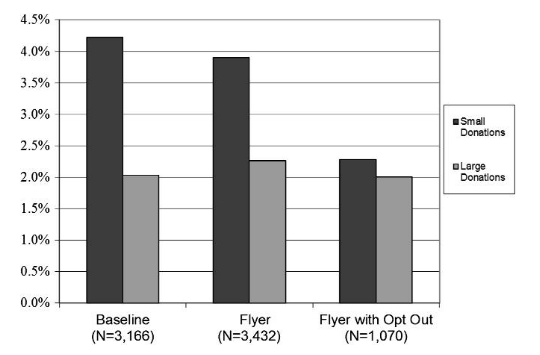
\includegraphics[width = .5\linewidth]{0821kato/fig8_2.png}
        \caption{Frequency of Giving: Small versus Large (Pooled)}
        \label{}
    \end{figure}

    \begin{itemize}
        \item 寄付金額の中央値である\$10がsocial pressure costを排除するための金額であると仮定する
        \begin{itemize}
            \item 少額寄付の割合:$\text{(no flyer)} > \text{(flyer)} > \text{(opt-out flyer)}$
            \item 高額寄付の割合:$\text{(no flyer)} = \text{(flyer)} = \text{(opt-out flyer)}$
        \end{itemize}
    \end{itemize}

    \subsection{Robustness}

    \begin{itemize}
        \item 説明変数や固定効果を変えても結果に大きな変化なし
        \item wave1-3に分けて分析した結果、一部異なる結果を得たが説明できる範囲内で収まった
        \begin{itemize}
            \item wave3 (2008 Sep-Oct):応答確率は似ていたが、寄付額が大きく下がった→リーマンショックと一致する時期
        \end{itemize}
    \end{itemize}

    \subsection{Survey Treatment}

    \begin{figure}[h]
        \centering
        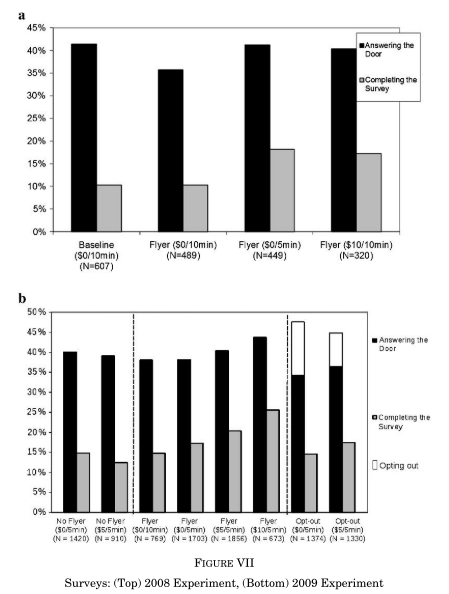
\includegraphics[width = .5\linewidth]{0821kato/fig9_2.png}
        %\caption{}
        \label{}
    \end{figure}

    \begin{itemize}
        \item 2008年の調査
        \begin{itemize}
            \item \$0/10min conditionのとき、応答確率は(no flyer) > (flyer) but not statistically significant
            \item flyer conditionのとき、時短調査や高謝礼調査は応答確率を高める but not statistically significant
        \end{itemize}
        \item 2009年の調査
        \begin{itemize}
            \item flyer conditionにおいて、応答確率とcomplete rateは時短や高謝礼によって上昇する
            \item 謝礼がないとき、opt-out flyerの応答確率はかなり減少する
        \end{itemize}
    \end{itemize}


    \section{Structural Estimation}

    \subsection{Models}

    \begin{itemize}
        \item 効用関数の定義
        \begin{align*}
            U(g, g_m) = (W - g) + a \log(\Gamma + g_i) - S*(10 - g_i)*1_{(g_i < 10)}, \quad
            a \sim N(\mu, \sigma | a > 0)
        \end{align*}
        \item 最適応答確率の目的関数
        \begin{align*}
            h[(W-g_i^*) + a \log(\Gamma + g_i^*) - S(10-g_i^*)1_{(g_i^* < 10)}] + (1 - h) W - \frac{(h - h_0)^2}{2\eta}
        \end{align*}
        \item サーベイ調査における最適応答確率の目的関数
        \begin{align*}
            h \max\{s + m - \tau v_s, -S^s\} - \frac{(h-h_0)^2}{2\eta}, \quad s \sim N(\mu^s, \sigma^s)
        \end{align*}
        \begin{itemize}
            \item $s$: 調査自体の効用
            \item $m$: 調査に対する謝金
            \item $\tau$:調査にかかる時間、$v_s$:1時間の価値
            \item $S^s$:サーベイ調査を断ることのsocial pressure cost
        \end{itemize}
    \end{itemize}

    \subsection{Moments}

    \begin{itemize}
        \item 推定するパラメータ
        \begin{align*}
            \xi = (h_0^{2008}, h_0^{2009}, r, \eta, \mu^s, \sigma^s, \v^s, S^s, \mu_a^{ch}, \sigma_a^{ch}, \Gamma, S^{ch}), \quad ch \in \{LaR, Ecu\}
        \end{align*}
        \begin{itemize}
            \item $h_0$:各年のno-flyer treatmentにおける応答確率
            \item $r$:flyerに気づく(覚えている)確率
            \item charity treatmentは寄付先ごとに推定する
        \end{itemize}
        \item モーメント
        \begin{align*}
            m(\xi) =& (P(H)_j^{ch}, P(OO)_{OO}^{ch}, P(G)_j^{ch}, P(0 < G < 10)_j^{ch}, P(G = g^s = 10)_j^{ch}, P(10 < G \le 20)_j^{ch}, \\
            & P(20 < G \le 50)_j^{ch}, P(G > 50)_j^{ch}, P(H)_k^s, P(SV)_k^s, P(OO)_k^s) ,\\
            &j = \{F, NF, OO\}
        \end{align*}
        \begin{itemize}
            \item $P(H)$:応答確率
            \item $P(OO)$:opt-outのチェックを入れる確率
            \item $P(G)$:寄付確率
            \item $P(SV)$:サーベイ調査を完了する確率
            \item $k$:$\text{incentive}\times\text{duration}\times\text{flyer condition}\times\text{survey year}$
        \end{itemize}
        \item パラメータはminimum-distance estimatorを使用する
        \begin{align*}
            \hat{\xi} \in \argmin_{\xi} (m(\xi) - \hat{m})'W(m(\xi) - \hat{m})
        \end{align*}
        \begin{itemize}
            \item 観察されるモーメント$\hat{m}$はreduced-formで使用したコントロール変数を用いて一段階目に推定する
            \item $W$は分散共分散行列の逆行列の対角要素を使用する(ロバスト分析に単位行列を使用) 
        \end{itemize}
    \end{itemize}

    \subsection{Source of Identification}

    \begin{itemize}
        \item $h_0$:観察される応答確率
        \item $r$:オプトアウトのチェックを入れた確率、応答確率
        \item $\eta$ (インセンティブに対する応答確率の弾力性):サーベイ調査の応答確率、寄付実験における各トリートメントの寄付額
        \item $\sigma_s, \mu_s$:各トリートメントのサーベイ達成率
        \item $v_s$:インセンティブの増加と時間減少による比較(何の?)
        \item $S^s$:サーベイ調査の応答確率
        \item $\sigma_a, \mu_a$:寄付額(特に$g > 10$の確率)
        \item $\Gamma$:寄付額($g < 10$の確率と$g > 10$の確率)
        \item $S^{ch}$:flyer treatmentにおける応答確率、$g < 10$の分布
    \end{itemize}


    \subsection{Estimates}

    \begin{figure}[h]
        \centering
        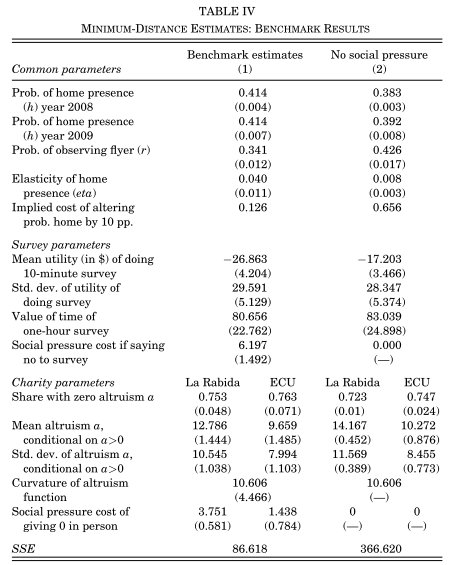
\includegraphics[width = .6\linewidth]{0821kato/fig10_2.png}
        %\caption{}
        \label{}
    \end{figure}

    \begin{itemize}
        \item これらは利他効用aの分布、hの費用関数の特定化やsocial pressureのheterogeneityを入れてもロバストな値として出てくる
        \item social pressureのコストが0のとき、モデルの精度(SSE)がかなり高くなっている⇒social pressureは行動を説明する重要な要素
    \end{itemize}

    \begin{figure}[h]
        \centering
        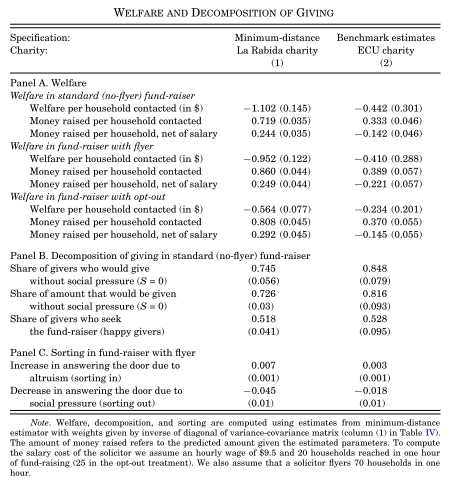
\includegraphics[width = .6\linewidth]{0821kato/fig11_2.png}
        %\caption{}
        \label{}
    \end{figure}

    \begin{itemize}
        \item La Rabidaに対するfundraising campaignは個人のwelfareを1.102ドル落とし、ECUに対するfundraising campaignは個人のwelfareを0.442ドル落とす
        \begin{itemize}
            \item La Rabidaのときのsocial pressure costが高いから
        \end{itemize}
        \item recipientのwelfareを加えて評価する際に寄付を集めるのにかかるコストを勧誘員の1世帯のあたりの時給とする
        \begin{itemize}
            \item La Rabidaでは0.244ドルだが、ECUでは-0.142ドル
        \end{itemize}
        \item flyer treatmentにおけるwelfareはno flyerのときよりも改善される
        \begin{itemize}
            \item 寄付したくない人がavoidする機会を提供し、寄付したい人は在宅するように心がけて高額の寄付をするから
            \item ECUについてrecipient sideを考慮したwelfareは改悪なことに注意(なぜ?)
        \end{itemize}
        \item opt-out flyerを用いたときのwelfareはさらに改善される
        \begin{itemize}
            \item flyerで考えられる効果に加えて、avoidするときのコストが取り除かれる
            \item また、勧誘員がチェックの入った世帯に訪問する必要がないので、一時間当たりで回れる世帯が多くなる
            \item recipient sideを考慮したwelfareがさらに改善される(ECUは改悪。なぜ?)
        \end{itemize}
        \item その他
        \begin{itemize}
            \item no-flyer conditionのとき、寄付した人のうち、寄付から得る効用が負の人はおよそ50\%
            \item flyerを受け取って、在宅確率を高める人は0.3 - 0.7程度増やすが、在宅確率を低くする人は1.8-4.5程度減らす
        \end{itemize}
    \end{itemize}


    \biblio

\end{document}